\documentclass[./main.tex]{subfiles}

\begin{document}

\chapter{Introduction}
Every person who has a desk job unconsciously is seated in an inconvenient
position for a prolonged duration. In the long run, these seating postures
might lead to undesirable health issues such as aches in the back and/or the
neck. Hence, this project aims to observe the posture of a person and notify
the duration of time for which the person was seated in a particular posture.
\\
This is achieved by:
\begin{itemize}
    \item Setting up a sensor-interfaced microcontroller to obtain the real-time data.
    \item Transmit the collected data points to a database.
    \item Classify the posture with the help of the data collected.
\end{itemize}

The following are the components used for data collection:
\begin{itemize}
    \item MPU6050 Gyro-Accelerometer
    \item Espressif's ESP8266
    \item Arduino UNO Microcontroller
\end{itemize}

\begin{figure}[H]
    \centering
    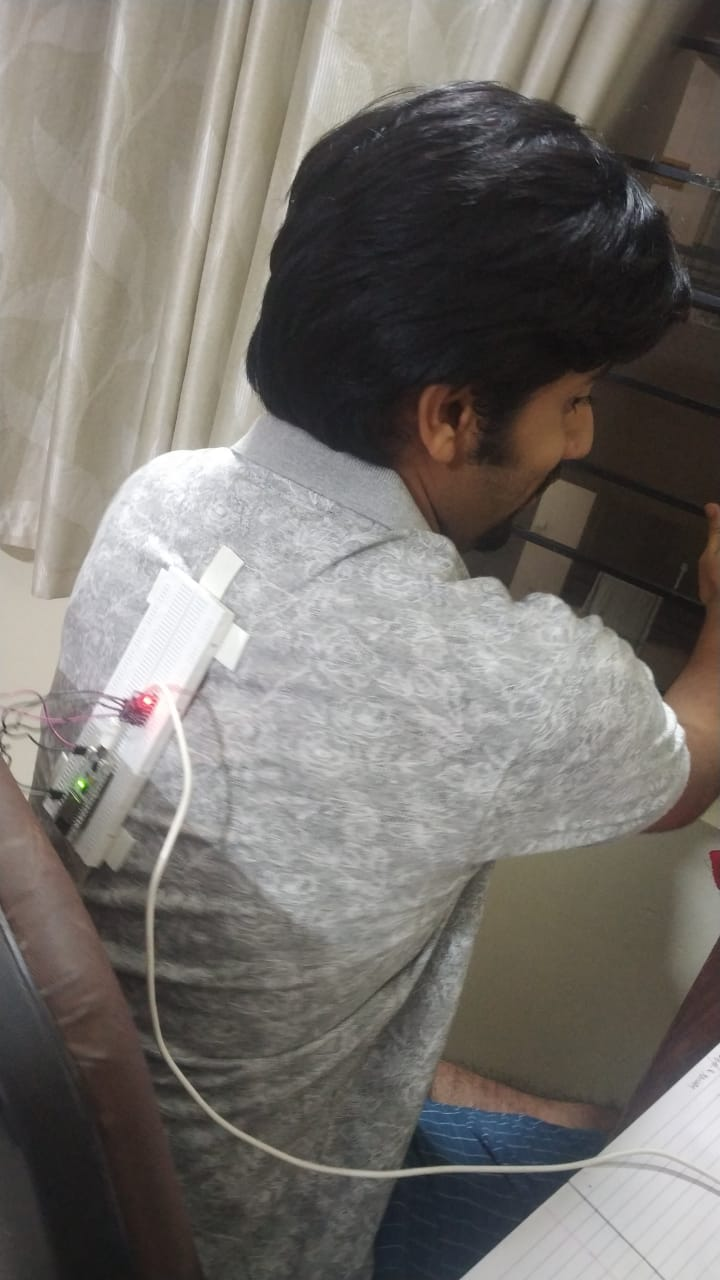
\includegraphics[scale=0.17]{data_collection.jpeg}
    \caption{Data collection setup}
    \label{fig:datacollect}
\end{figure}

The module has to be attached on the back for data collection and this data is
also plotted in real-time for visualization purposes and finer interpretation.
\end{document}
